% ============================================================
% CHAPITRE 6
% ============================================================
\chapter{Le lakehouse Delta : historiser et auditer}
\label{ch:lakehouse}

\section{Une architecture médaillon en sept tables}
L'énoncé demande l'historisation complète des sous-graphes d'anomalies, sous
Delta Lake, partitionnée par \fichier{risk\_level} et par jour. Le lakehouse
suit l'organisation « médaillon » (figure~\ref{fig:medaillon}) : le
\motcle{bronze} garde les transactions telles qu'elles ont été acceptées, le
\motcle{silver} des données consolidées pour l'analyse, le \motcle{gold} les
alertes et leurs sous-graphes, c'est-à-dire la piste d'audit. Les sept
définitions de tables vivent dans un seul fichier,
\fichier{fraud\_graph\_delta\_schema.py}, qui sait aussi imprimer le DDL
complet (annexe~\ref{ann:ddl}).

\begin{figure}[htp]
\centering
\begin{tikzpicture}[
  couche/.style={rounded corners=4pt, draw=#1, line width=1pt, fill=#1!7, minimum width=4.75cm,
    minimum height=4.6cm},
  titre/.style={font=\sffamily\small\bfseries, color=#1},
  t/.style={draw=#1, fill=white, rounded corners=2pt, font=\ttfamily\tiny, text width=4.15cm, inner sep=3pt,
    align=left},
  prop/.style={font=\sffamily\tiny, color=encre2, text width=4.3cm, align=left}]
  \foreach \x/\c/\nom/\role in {0/bleuprojet/Bronze/{brut validé}, 5.2/cat3/Silver/{consolidé}, 10.4/orangeprojet/Gold/{métier, audit}} {
    \node[couche=\c] at (\x,0) {};
    \node[titre=\c] at (\x,2.0) {\nom};
    \node[font=\sffamily\tiny, color=encre2] at (\x,1.65) {\role};
  }
  \node[t=bleuprojet] at (0,0.85) {\textbf{transactions}\\{\sffamily partition : dt}\\{\sffamily CHECK montant > 0, pas d'auto-virement}};
  \node[t=bleuprojet] at (0,-0.35) {\textbf{transactions\_quarantine}\\{\sffamily message brut + motif du rejet}};
  \node[t=cat3] at (5.2,0.85) {\textbf{account\_metrics}\\{\sffamily PageRank, degrés, flux, SCC, cluster par compte et par instantané}};
  \node[t=cat3] at (5.2,-0.35) {\textbf{traffic\_windows}\\{\sffamily fenêtres 10 min / 1 min, MERGE}};
  \node[t=orangeprojet] at (10.4,0.95) {\textbf{fraud\_alerts}\\{\sffamily type, score, niveau, comptes, transactions, explication}};
  \node[t=orangeprojet] at (10.4,-0.05) {\textbf{anomaly\_subgraph\_vertices}\\{\sffamily comptes et rôle (ORIGINE, MULE, PIVOT\ldots)}};
  \node[t=orangeprojet] at (10.4,-0.95) {\textbf{anomaly\_subgraph\_edges}\\{\sffamily virements du sous-graphe}};
  \node[prop] at (0,-1.75) {rétention du journal : 30 jours\\écrit par le chemin rapide, \emph{après} gold};
  \node[prop] at (5.2,-1.75) {rétention du journal : 30 jours\\écrit par le chemin lent et la requête de trafic};
  \node[prop] at (10.4,-1.85) {partitions \fichier{risk\_level / dt}\\\fichier{appendOnly} : aucune modification\\journal conservé 365 jours};
  \draw[-{Stealth[length=2.2mm]}, line width=1pt, color=grismoyen] (2.45,0) -- (2.75,0);
  \draw[-{Stealth[length=2.2mm]}, line width=1pt, color=grismoyen] (7.65,0) -- (7.95,0);
\end{tikzpicture}
\caption[Le lakehouse médaillon]{Les sept tables du lakehouse, leurs contraintes et leurs propriétés.}
\label{fig:medaillon}
\end{figure}

\begin{table}[htp]
\centering\small
\begin{tabular}{@{}>{\ttfamily}l>{\ttfamily}l>{\raggedright\arraybackslash}p{8.6cm}@{}}
\toprule
\multicolumn{1}{@{}l}{\sffamily\bfseries Colonne} & \multicolumn{1}{l}{\sffamily\bfseries Type} & \sffamily\bfseries Rôle\\
\midrule
alert\_id & STRING & empreinte déterministe du type et des clés : rejouer un lot redonne le même identifiant\\
alert\_type & STRING & CYCLE, CYCLE\_LONG, MULE, SCATTER\_GATHER, PIVOT, CLUSTER\\
risk\_score, risk\_level & INT, STRING & score 0--100 (contrainte) et niveau ; \fichier{risk\_level} est une clé de partition\\
accounts, transaction\_ids & ARRAY & les comptes et les virements du schéma\\
window\_start, window\_end & TIMESTAMP & première et dernière transaction du motif\\
detected\_at, latency\_ms & TIMESTAMP, BIGINT & heure de détection et délai depuis l'ingestion Kafka\\
explanation, features & STRING & explication en français et indicateurs du score (JSON)\\
detector, dt & STRING & \fichier{fast-path} ou \fichier{slow-path} ; jour (clé de partition)\\
\bottomrule
\end{tabular}
\caption{Schéma de la table \fichier{gold/fraud\_alerts}.}
\label{tab:schemaalertes}
\end{table}

\section{Le lakehouse après les runs}
La figure~\ref{fig:delta} montre le lakehouse « vivre » pendant le run
d'évaluation : la table bronze reçoit un commit par micro-batch (près de 500
en 40~minutes), compacté périodiquement par \fichier{OPTIMIZE} pour éviter
l'accumulation de petits fichiers ; la table des alertes se répartit entre
ses partitions de niveau de risque.

\begin{figure}[htp]
\centering
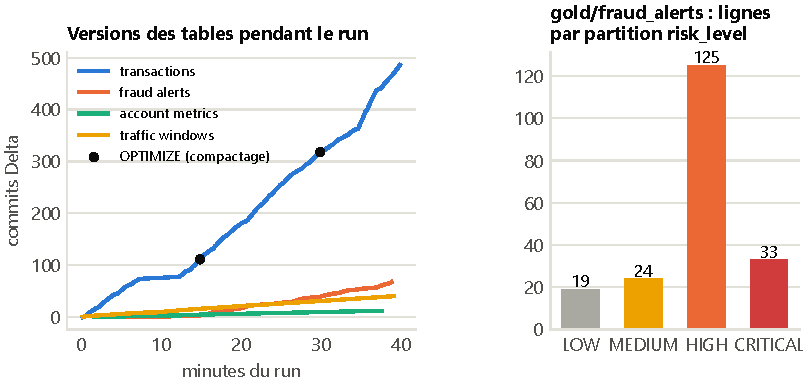
\includegraphics[width=\linewidth]{figures/delta_tables.pdf}
\caption[Les tables Delta pendant le run]{À gauche, versions des tables pendant le run d'évaluation
(journal \fichier{\_delta\_log}). À droite, contenu des partitions \fichier{risk\_level} de la table
des alertes à la fin de tous les runs (201 alertes).}
\label{fig:delta}
\end{figure}

\begin{figure}[htp]
\centering
\begin{tikzpicture}[
  dossier/.style={font=\ttfamily\scriptsize, anchor=west, inner sep=1pt},
  info/.style={font=\sffamily\tiny, color=encre2, anchor=west}]
  \node[dossier] (r) at (0,0) {\ico{F07C}~gold/fraud\_alerts/};
  \node[dossier] at (0.5,-0.45) {\ico{F15C}~\_delta\_log/ \hspace{0.3cm}{\sffamily\tiny\color{encre2} 132 versions, chaque commit = un fichier JSON}};
  \foreach \lvl/\n/\c [count=\i] in {LOW/19/grismoyen, MEDIUM/24/cat4, HIGH/125/orangeprojet, CRITICAL/33/critique} {
    \node[dossier] (l\i) at (0.5,-0.45-\i*0.45) {\color{\c}\ico{F07B}~risk\_level=\lvl/};
    \node[dossier] at (4.0,-0.45-\i*0.45) {\ico{F07B}~dt=2026-11-18/};
    \node[info] at (7.0,-0.45-\i*0.45) {\n~alertes};
  }
  \draw[grismoyen] (0.3,-0.2) -- (0.3,-2.25);
  \node[font=\sffamily\scriptsize, text width=5.4cm, align=left, anchor=west] at (8.6,-1.2) {Une requête « alertes CRITICAL
  d'aujourd'hui » ne lit qu'un dossier : c'est l'intérêt du partitionnement imposé par l'énoncé
  (\emph{partition pruning}).};
\end{tikzpicture}
\caption{Organisation physique de la table des alertes.}
\label{fig:partitions}
\end{figure}

\section{Exactly-once : une alerte une seule fois, même après une panne}
Un système d'alerte qui envoie deux fois la même alerte perd la confiance des
analystes ; un lakehouse d'audit qui contient des doublons perd sa valeur de
preuve. Spark garantit qu'un micro-batch est rejoué en entier après une panne,
mais \emph{pas} que ses effets externes n'aient pas déjà eu lieu en partie.
La plateforme combine donc trois mécanismes (figure~\ref{fig:exactlyonce}).

\begin{figure}[htp]
\centering
\begin{tikzpicture}[
  w/.style={draw=#1, line width=0.9pt, fill=#1!10, rounded corners=3pt, minimum width=2.35cm,
    minimum height=0.85cm, font=\sffamily\scriptsize, align=center},
  crash/.style={font=\sffamily\small, color=critique}]
  \node[w=grismoyen] (d) at (0,0) {détection\\{\tiny alert\_id = empreinte}};
  \node[w=orangeprojet] (k) at (3.4,0) {1 · Kafka\\{\tiny fraud-alerts}};
  \node[w=orangeprojet] (g) at (6.8,0) {2 · Delta gold\\{\tiny alertes + sous-graphes}};
  \node[w=bleuprojet] (b) at (10.2,0) {3 · Delta bronze\\{\tiny transactions}};
  \node[w=vertcode] (c) at (13.4,0) {commit du\\checkpoint};
  \foreach \a/\b in {d/k, k/g, g/b, b/c} \draw[fleche] (\a) -- (\b);
  \foreach \x/\txt in {1.7/{rejeu : même alerte, même \fichier{alert\_id}}, 5.1/{rejeu : gold ignore le doublon (\fichier{txnVersion})}, 8.5/{rejeu : bronze ignore le doublon (\fichier{txnVersion})}, 11.8/{rien à rejouer}} {
    \node[crash] at (\x,0.75) {\ico{F0E7}};
    \node[font=\sffamily\tiny, color=encre2, text width=2.9cm, align=center, anchor=north] at (\x,-0.55) {\txt};
  }
  \node[font=\sffamily\tiny\bfseries, color=critique, anchor=west] at (-1.3,0.75) {panne ici :};
\end{tikzpicture}
\caption[Ordre des écritures et reprise après panne]{Ordre des écritures d'un micro-batch et effet d'une
panne à chaque étape. Le seul doublon possible est côté Kafka, où le consommateur le reconnaît à son
\fichier{alert\_id} ; l'audit Delta reste exact.}
\label{fig:exactlyonce}
\end{figure}

\begin{itemize}
\item \textbf{Identifiants déterministes.} L'\fichier{alert\_id} est une empreinte du type et des
clés de l'alerte (transactions d'un cycle ; compte et jour d'une mule ou d'un pivot ; source,
destination et jour d'un scatter-gather). Redétecter la même fraude redonne le même identifiant.
\item \textbf{Écritures Delta idempotentes.} Chaque écriture porte le couple \fichier{txnAppId} /
\fichier{txnVersion} (identifiant de la requête, numéro du lot) : Delta ignore une écriture déjà
validée pour ce couple.
\item \textbf{Mémoire des alertes émises.} Le chemin lent, qui revoit les mêmes schémas à chaque
passage, garde l'ensemble des identifiants déjà émis, reconstruit depuis gold au démarrage.
\end{itemize}

\section{Le test de panne}
Le test rejoue la situation la plus défavorable : Spark est tué brutalement
(\fichier{docker compose kill}, équivalent d'un \fichier{kill -9}) en pleine
ingestion, pendant que le producteur continue d'écrire dans Kafka. Il est
redémarré 48~secondes plus tard ; on vérifie ensuite l'intégrité du
lakehouse (figure~\ref{fig:panne} et tableau~\ref{tab:integrite}).

\begin{figure}[htp]
\centering
\begin{tikzpicture}[x=0.0265cm]
  \draw[grismoyen, line width=0.8pt] (0,0) -- (556,0);
  \fill[orangeclair] (240,-0.18) rectangle (288,0.18);
  \fill[grisligne] (288,-0.18) rectangle (470,0.18);
  \foreach \t/\c in {0/bleuprojet, 240/critique, 288/orangeprojet, 470/vertcode, 556/vertcode}
    \fill[\c] (\t,0) circle (1.3mm);
  \tikzset{hh/.style={font=\sffamily\tiny\bfseries, color=#1}, xx/.style={font=\sffamily\tiny, align=center}}
  \node[hh=bleuprojet, anchor=south] at (0,0.15) {21:37:20};
  \node[xx, anchor=north, text width=2.6cm] at (0,-0.2) {démarrage de Spark et du producteur};
  \node[hh=critique, anchor=south] at (240,0.15) {21:41:20};
  \node[xx, anchor=north east, text width=1.7cm, align=right] at (246,-0.2) {\textbf{kill} de Spark};
  \node[hh=orangeprojet, anchor=north] at (288,-0.15) {21:42:08};
  \node[xx, anchor=south west, text width=1.6cm, align=left] at (282,0.2) {redémarrage};
  \node[hh=vertcode, anchor=south] at (470,0.15) {21:45:10};
  \node[xx, anchor=north, text width=2.8cm] at (470,-0.2) {état reconstruit : 22\,695 arêtes, 191 alertes connues};
  \node[hh=vertcode, anchor=north] at (556,-0.15) {21:46:36};
  \node[xx, anchor=south, text width=2.0cm] at (556,0.2) {contrôle d'intégrité};
\end{tikzpicture}

\vspace{4mm}
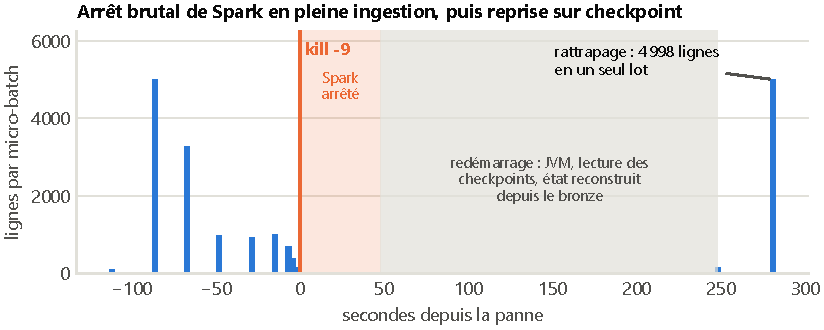
\includegraphics[width=\linewidth]{figures/panne_reprise.pdf}
\caption[Le test de panne]{Le test de panne (heures UTC). Au redémarrage, Spark relit ses checkpoints,
reconstruit son état en mémoire depuis le bronze (graphe glissant, journal des dépôts, alertes déjà
émises) puis rattrape d'un coup les messages accumulés dans Kafka.}
\label{fig:panne}
\end{figure}

\begin{table}[htp]
\centering\small
\begin{tabular}{@{}>{\raggedright\arraybackslash}p{8.5cm}rc@{}}
\toprule
\sffamily\bfseries Contrôle (\fichier{scripts/check\_integrity.py}) & \sffamily\bfseries Résultat & \\
\midrule
Transactions en double dans le bronze (même \fichier{transaction\_id}) & 0 & \oui\\
Transactions violant les contraintes métier & 0 & \oui\\
Alertes en double dans le gold (même \fichier{alert\_id}) & 0 & \oui\\
Sous-graphes sans alerte (orphelins) & 0 & \oui\\
\midrule
Transactions dans le bronze / alertes dans le gold & 201\,934 / 198 & \\
\bottomrule
\end{tabular}
\caption{Contrôle d'intégrité du lakehouse après la panne.}
\label{tab:integrite}
\end{table}

\aretenir{À retenir}{L'ordre des écritures (Kafka, puis gold, puis bronze), des identifiants
déterministes et les transactions idempotentes de Delta donnent une historisation
\emph{exactly-once} : après un arrêt brutal, aucune transaction ni aucune alerte n'est dupliquée.}
